%aum ghanaathipathaye namaha
%sri rama jeyam

\section{Computation Modelling} \label{subsec:abs_sem_mod}
The key problem in state-based semantic modelling is that it is too low-level, which may lead to the same semantics model from totally different binary codes.
Therefore, matching using state-based semantic information will give too many false positives, especially when the program segment is small.
In addition, as explained in previous section, with the presence of an uninterpreted system API, the state-based semantic models are incapable of capturing the precise semantics. In fact, it is impossible to model the machine state transitions involving system API using static analysis unless the semantic summaries are available for all system APIs.

To complement state-based semantic modeling, we introduce an idiom based computation modeling to capture the high level computation (or behaviour), including the system APIs.
To this end, we leverage on two types of analysis to infer the high-level computation: (1) machine code \textit{idiom analysis}, and (2) \textit{idiom dependency analysis}. Idiom analysis try to look for familiar and recurring machine code patterns that are already observed in the majority of the binaries in the wild, whereas, idiom dependency analysis captures the relationship (i.e., dependency) between the extracted idioms.

%In addition, even if the program segment is free of any uninterpreted system API, if it is too small, i.e., too few instructions, the state-based models will become unreliable, where two totally irrelevant code segments might result in an identical post-state (i.e., machine state after execution) given the same pre-state (i.e, machine state before execution)

%\begin{figure}[!h]
%\scriptsize
%  \begin{subfigure}[b]{0.5\linewidth}
%    \centering
%   % \includegraphics[width=0.75\linewidth]{srj-figures/srj-hierarchy-2.png}
%    \raggedright{\textbf{\texttt{
%    \\
%    	add  ebx, eax\\
%    	add  ebx, 2h\\
%   		shl  ebx, 2\\
%   		test ebx, 4\\
%   		jz ecx\\
%    }}}
%    \caption{\small{}}
%   \label{fig:traceleta}
%    \vspace{1ex}
%  \end{subfigure}%%
%  \begin{subfigure}[b]{0.5\linewidth}
%    \centering
%      \raggedright{\textbf{\texttt{
%    \\
%    	mov eax, [0x1234]\\
%    	lea	ebx, [eax+0x4]\\
%   		mov	eax, [ebx]\\
%   		cmp eax, 0\\
%   		jz edx\\
%    }}}
%    \caption{\small{}}
%    \label{fig:traceletb}
%    \vspace{1ex}
%  \end{subfigure}
%  \caption{Code segments that result in identical post-state given the same pre-state even though their high-level intentions are not comparable\\}
%  \label{fig:ex-tracelet}
%\end{figure}
%
%For example, given the same pre-state, the code segments given in figure~\ref{fig:abs} will result in an identical post-state even though their high-level intentions are not comparable. That is, assuming all the registers, flags and memory locations are assigned the value `0' in the pre-state. After execution, the post-state for code segment (a) will be: \texttt{ebx} register will hold the value `4', while all other registers, flags and memory locations will retain their pre-state values. Similarly, in the post-state for code segment (b), the \texttt{ebx} register will hold the value `4' and all the other registers, flags and memory locations will retain their pre-state values.

%This behaviour is undesirable especially, when searching for potential vulnerable code segments in the target binary, where this will lead to high false positive rate. Hence, in \tool, we complement state-based models with abstract semantic models, where state-based models capture the low-level semantics of the code segment and using abstract semantic models we try to capture the high-level objective (or behaviour) of the code segment. The features extracted from these two models are complement to each other.
%To this end, we leverage on two types of analysis to infer the high-level computations of the code segments: (1) machine code \textit{idiom analysis}, and (2) \textit{dependency analysis}. Idiom analysis try to look for familiar and recurring machine code patterns that are already observed in the majority of the binaries in the wild, whereas, dependency analysis captures the relationship (i.e., dependency) between the extracted idioms.

%As discussed in section~\ref{sec:prob_state}, program segments (or functions) perform a series of computations through which they accomplish their objectives (e.g., create a buffer in the memory, send data over network). To understand the high-level objective (or behaviour) of a program segment, it is essential to capture the computations underneath it.

\subsection{Idioms} \label{subsec:idiom_ana}
Motivated by source code idioms~\cite{allamanis2014mining}, we find that the same concept applies in binaries, i.e., the recurring patterns of binary instructions reveal some fixed semantics.
%The presence of idioms, in the program segment, helps to understand the machine code better.
For example, the idiom given below, indicates that the code segment under analysis sets up the stack frame in the function prologue.
\begin{itemize}
\centering
\itemsep-0.5em
  \item[] $\mathtt{push \;\;ebp; \quad mov \;\; ebp, esp;}$
 % \item[] $\mathtt{mov \quad ebp, esp}$
\end{itemize}

In addition to revealing high-level behaviour, idioms can also explain the compilation process.
The presence of code fragments below in the function prologue and epilogue ensure that the stack integrity is not violated, where it is automatically included by the compiler (in this case, $\mathtt{gcc}$) when stack smash protection compiler feature is enabled (using either -$\mathtt{fstack}$-$\mathtt{protector}$-$\mathtt{all}$ or -$\mathtt{fstack}$-$\mathtt{protector}$ flag) during program compilation. Generalizing the above code segments into an idiom helps an analyst to identify functions that are protected by stack smash protection (SSP) compiler feature\footnote{Stack smash protection is a first line of defence that merely detects the stack buffer over runs and does not prevent them. This protection can be beaten by correctly identifying the stack canary~\ref{pincus2004beyond}.}. %Hence, idioms can also be used to pre-filter the candidate target functions that are of analyst's interest.
%help in pre-filtering the target candidates, especially in vulnerability signature matching. For example, consider the following program segment:
\begin{itemize}
%\centering
\itemsep-0.2em
  \item[] $\mathtt{mov  \quad eax, gs:20 \quad}$
  \item[] $\mathtt{mov \quad [ebp-12], eax}$
  \makebox(0,0){\put(0,2.2\normalbaselineskip){%
               $\left.\rule{0pt}{1.1\normalbaselineskip}\right\}$ function prologue}}
  \item[] $\mathtt{\ldots \quad\quad\quad}$
  \item[] $\mathtt{\ldots\quad\quad\quad}$
  \item[] $\mathtt{mov  \quad eax, [ebp-12]}$
  \item[] $\mathtt{xor \quad eax, gs:20 \quad\quad}$
  \makebox(0,0){\put(0,2.2\normalbaselineskip){%
               $\left.\rule{0pt}{1.1\normalbaselineskip}\right\}$ function epilogue}}
\end{itemize}

%in addition to understand the high-level behaviour,

Hence, using idioms, we can capture various interesting properties in a program segment, which in return, help us to understand the high-level behaviour. We formally define idiom as follows:

%\ly{machine code below is same as the instructions in sec 4? or QFBV? make sure the consistancy} \note{This is pure machine code. QFBV is redundant. I'll remove QFBV in sec 4}
\begin{mydef}
\emph{(\textbf{Idiom})} is a recurring machine code pattern that has a single semantic purpose, which may be unified across different architectures and platforms.
\end{mydef}

We want to look for machine code patterns (i.e., instruction sequences) that are frequently observed in the wild binaries and map them to meaningful unified high-level constructs, if there is one. It is critical to note that the instruction sequences are architecture and platform dependent, however, their high-level objectives (i.e., the tasks achieved by the instruction sequences) are, in general, agnostic to differences in architecture and platform. For example, the instruction sequence require to invoke a system API in one architecture is totally from another depending on the calling conventions used (discussed in section xx), however, at high-level they are all achieving the same objective of invoking the same or similar system API.
%\note{Similarly, the system APIs too unified based on the objectives accomplished}
%\note{Similarly, the system APIs, that are used to accomplish similar objectives, can vary from OS (or platform) to OS and between different versions of the same OS, hence they too need to be abstracted}.
Therefore extracting idioms, from various architectures and platforms, with mapping to a unified high-level meaning helps to summarize the semantics of the program segment (or function) under analysis.
\ly{Note that some idioms may be environment specific, e.g., . We argue that these idioms are also useful, e.g., to filter the relevant idioms to fast matching.}


%An idiom is a syntactic fragment that recurs  frequent across binaries and has a single semantic purpose \cite{allamanis2014mining}.
\subsubsection{Idiom Classification}
The high level computation model of a binary program, in general, can be characterised by various concepts such as data structures used (e.g., array, structure, $\ldots$), data type information (e.g., \texttt{int}, \texttt{float}, $\ldots$), variable types involved (e.g., local and global variables), system APIs invoked during the computation (e.g., \texttt{strlen}, \texttt{memcpy}, $\ldots$), and other structural properties. In addition, compiler too, sometimes, influence a computation through its various compiler features such as stack smash protection (using \texttt{-fstack-protector} flag in \texttt{gcc}).

\ly{need to give one example for each type} \note{will update in table 2}
To reflect different aspect of the high level computation, 
in this work, we classify the idioms into three major classes based on the nature of information extracted: (1) semantic idioms, (2) structural idioms, and (3) compiler idioms. 

%
%\begin{itemize}
%
%\item \textbf{Semantic idiom}: This type of idioms provide the semantic details of the code segment under analysis, where it captures the system API invocation patterns. System API, in general, indicates the type of operation carried out by the program. For example, presence of \texttt{strlen} system API indicates that the program handles strings, more specifically, string arithmetic. In addition, co-occurrence of two or more system API gives more insight into the high-level intentions of the program segment. For instance, presence of \texttt{strlen} and \texttt{memcpy} system APIs in a code segment indicates buffer manipulation operation involving string arithmetic. Hence, learning the system API invocation patterns from existing binaries and generalizing them in to meaningful semantic idioms will help analysts to understand the high-level intentions of binary programs under evaluation.  It is important to note that to accommodate cross-platform analysis, we apply two levels of abstraction for system APIs (discussed in detail later in the section).
%
%\item \textbf{Structural idiom}: These idioms helps to identify the structural details and code properties of the program segment. For example, presence of an instruction pattern \texttt{sub esp,Imm} in a code segment compiled for \texttt{x86 32-bit} architecture indicates stack frame size manipulation operation. In addition, also capture other common structural properties such as save/restoring of callee/caller-save registers\footnote{Callee-saved registers are used to hold long-lived values that should be preserved across calls. Similarly, caller-saved registers are used to hold temporary quantities that need not be preserved across calls.}, presence of function prologue/epilogue and presence of loops. Further structural idioms also try to capture the code properties such as local/global variable access, function parameter manipulation and array manipulation.  It is important to note that structural idioms are architecture dependent, however, their high-level meanings are unified across architectures. Further, one cannot precisely extract code properties using structural idioms, for example, using only light-weight static analysis, it is impossible to distinguish between a string and an array\footnote{\note{mention how they are represented in memory}}. However, in our analysis, if there is a consecutive memory access pattern, we try to guess the data structure based on the co-occurrence of other idioms, that is, we map consecutive memory access pattern to a string given the presence of string related system APIs in the code segment. This approach is not precise but works relatively well and very scalable compare to more heavy-weight program analysis techniques~\cite{balakrishnan2007divine}.
%
%\item \textbf{Compiler idiom}: These idioms helps to identify the additional code included by the compiler during compilation process. For example, there are more than \note{XX} compiler options available for \texttt{gcc} that a programmer can choose from when compiling her code, where most of the features insert additional code into the compiled binary. One such example is the stack smash protection (SSP) code included in the function prologue and epilogue. Interestingly, some compiler idioms helps to understand more about the program, for example, presence of SSP in selected functions (i.e., -$\mathtt{fstack}$-$\mathtt{protector}$ compiler feature) in a program indicates that those functions have buffers larger than 8 bytes. It is also noted that the compiler idioms are architecture and platform specific, however, their high-level meanings are unified across architectures and platforms.
%\end{itemize}

\noindent \textbf{Semantic Idiom}
This type of idioms provides the semantic details of the code segment under analysis, where it captures the system API invocation patterns. System API, in general, indicates the type of operation carried out by the program. For example, presence of \texttt{strlen} system API indicates that the program handles strings, more specifically, string arithmetic. In addition to extracting the system API, it is observed that identifying the co-occurrence of two or more system API gives more insight into the high-level behaviour of the program segment. For example, presence of \texttt{strlen} and \texttt{memcpy} system APIs in a code segment indicates buffer manipulation operation involving string arithmetic.

It is important to note that one can simply look for \texttt{call} instruction mnemonic (in x86) to identify the call invocations. Unfortunately, there are alternative ways to invoke a function without using \texttt{call} instruction~\cite{lakhotia2004abstracting}. For example, \texttt{call} instruction can be replaced by \texttt{push}/\texttt{jmp} or \texttt{push}/\texttt{ret} instruction sequences as shown in Fig.~\ref{fig:altr_call_ins}.
%To this end, we use idioms to identify the possible instruction sequences that are used to invoke system APIs.

\begin{figure}[t]
\scriptsize
  \begin{subfigure}[b]{0.5\linewidth}
    \centering
   % \includegraphics[width=0.75\linewidth]{srj-figures/srj-hierarchy-2.png}
    \raggedright{\textbf{\texttt{
    \\
    	push  next\_instr\\
    	jmp  some\_func\\
   		//next\_instr\\
    }}}
    \caption{Using \texttt{push}/\texttt{jmp} instructions}
   %\label{fig:traceleta}
    \vspace{1ex}
  \end{subfigure}%%
  \begin{subfigure}[b]{0.5\linewidth}
    \centering
      \raggedright{\textbf{\texttt{
      \\
   		push  next\_instr\\
    	push  some\_func\\
    	ret\\
   		//next\_instr\\
    }}}
     \caption{Using \texttt{push}/\texttt{ret} instructions}
    %\label{fig:traceletb}
    \vspace{1ex}
  \end{subfigure}
  \caption{Alternative ways to invoke a function. Assume the function \texttt{some\_func} doesn't take any input parameters.}
  \label{fig:altr_call_ins}
\end{figure}

\noindent Hence, learning the possible system API invocation patterns from existing binaries and generalizing them in to meaningful semantic idioms will help the analysts to understand the high-level behaviour of binary programs under evaluation.  Further, to accommodate cross-platform analysis, we also apply two levels of abstraction for system API. That is, different APIs can be used to accomplish the same objective in different platforms (e.g., Windows vs. Linux) or in different versions of the same platform (e.g., Windows XP vs. Windows 7), hence, an abstraction process is used to unify the system APIs across platforms and versions (discussed more in Section xx).

\noindent \textbf{Structural idiom}
These idioms helps to identify the structural details and code properties of the program segment. For example, presence of an instruction pattern \texttt{sub esp,Imm} in a code segment compiled for \texttt{x86 32-bit} architecture indicates stack frame size manipulation operation. In addition, also capture other common structural properties such as save/restoring of callee/caller-save registers\footnote{Callee-saved registers are used to hold long-lived values that should be preserved across calls. Similarly, caller-saved registers are used to hold temporary quantities that need not be preserved across calls.}, presence of function prologue/epilogue and presence of loops. Further structural idioms also try to capture the code properties such as local/global variable access, function parameter manipulation and array manipulation.  It is important to note that structural idioms are architecture dependent, however, their high-level meanings are unified across architectures. Further, one cannot precisely extract code properties using structural idioms, for example, using only light-weight static analysis, it is impossible to distinguish between a string and an array\footnote{\note{mention how they are represented in memory}}. However, in our analysis, if there is a consecutive memory access pattern, we try to guess the data structure based on the co-occurrence of other idioms, that is, we map consecutive memory access pattern to a string given the presence of string related system APIs in the code segment. This approach is not precise but works relatively well and very scalable compare to more heavy-weight program analysis techniques~\cite{balakrishnan2007divine}.

\noindent \textbf{Compiler idiom}
These idioms helps to identify the additional code included by the compiler during compilation process. For example, there are more than \note{XX} compiler options available for \texttt{gcc} that a programmer can choose from when compiling her code, where most of the features insert additional code into the compiled binary. One such example is the stack smash protection (SSP) code included in the function prologue and epilogue. Interestingly, some compiler idioms helps to understand more about the program, for example, presence of SSP in selected functions (i.e., -$\mathtt{fstack}$-$\mathtt{protector}$ compiler feature) in a program indicates that those functions have buffers larger than 8 bytes. It is also noted that the compiler idioms are architecture and platform specific, however, their high-level meanings are unified across architectures and platforms.

\subsubsection{Idiom Dependency} \label{subsec:dep-ana}

In the previous section, we discussed how the high-level behaviour of a program segment can be summarized using idioms. However, it is even interesting and useful to identify the relationship (or dependency) among idioms.
It is important to note that the idiom co-occurrence matrix generated from Algorithm \ref{algo:idiom-ext} just tell whether two idioms present together in a program segment, however, it does not tell anything about the dependency among the co-occurring idioms. The dependency analysis can play a vital role in signature matching, \note{where it helps to capture the precise semantics of the binary code}.

\note{In addition, the dependency details among idioms can be very handy for security analysts, where it enables them to utilize their expertise in improving the search results. That is, the security analyst can specify additional constraints (or useful hints) that are not explicitly visible in the vulnerability signature. For example, by leveraging on the idiom dependency, security analyst can determine whether a global (or static) variable (captured by structural idiom) is passed to a system API (captured by semantic idiom) or whether there is a dependency between two sensitive system APIs (e.g., \texttt{strlen} and \texttt{memcpy}).} To this end, we first identify the data dependency among instruction sequence using def-use chain \cite{} and later, identify the idioms present along the data-flow. \note{That is, idioms are marked as dependent, if they fall along the data-flow path. The algorithm to identify idiom dependency is presented in Section~\ref{subsubsec:dep_cal}}.


\begin{MyAlgo}[!ht]{-4.9cm} %increase or decrease margin, span across columns
 \DontPrintSemicolon
 \KwData{binary corpus $\beta$}
 \KwResult{set of idioms $\Re$, idioms co-occurrence matrix $\Re_M$}
% \SetKwFunction{algo}{ExtractTracelets}\SetKwFunction{proc}{Extract}
% \SetKwProg{myalg}{Algorithm}{}{}
% \myalg{\algo{$CFG$}}{
   $\Re \longleftarrow \emptyset$ \;
   $\Re_M \longleftarrow \emptyset$ \;
   $\mathtt{dict[\cdot]=\lbrace\rbrace}$ \tcp*{n-gram dictionary}
   \ForEach{{\upshape binary} b {\upshape in} $\beta$}{
   $ F := \mathtt{getFunctions}(b)$\;
   $ F_n := \mathtt{normalizeFunctions}(F)$ \tcp*{algorithm \ref{algo:norm}}
   $ \wp := \mathtt{getPartialTraces}(F_n)$ \tcp*{algorithm \ref{algo:k-trace}}
    \ForEach{{\upshape partial trace} p {\upshape in} $\wp$}{
     	\ForEach{n = {\upshape 1 \textbf{To}} $\mathtt{MAX}$}{
   			$ S_n := \mathtt{getNgramModel}(p, n)$\;
   			$ \mathtt{updateDict}(\mathtt{dict_n}, S_n)$\;
   		}
   	}
   }
   \tcp{extract idioms based on a threshold value $t$}
   $\Re := \mathtt{getIdioms}(\mathtt{dict},t)$ \tcp*{manual vetting involved}
   $\Re_M := \mathtt{getIdiomCoOccurrenceMatrix}(\Re,F_n)$\;
  \Return ${\Re, \Re_M}$
  \\
 \caption{Idiom extraction from binary programs}\label{algo:idiom-ext}
\end{MyAlgo}

{\SetInd{0.4em}{0.5em}
\begin{MyAlgo}[!ht]{-4.9cm} %increase or decrease margin, span across columns
 \DontPrintSemicolon
 \KwData{Set of  control-flow graphs, $CFG$}
 \KwResult{Set of normalized control-flow graphs, $CFG_n$}
% \SetKwFunction{algo}{ExtractTracelets}\SetKwFunction{proc}{Extract}
% \SetKwProg{myalg}{Algorithm}{}{}
% \myalg{\algo{$CFG$}}{
   $CFG_n \longleftarrow \langle\rangle$ \;%\tcp*{set of abstract semantic graphs}
   %$\mathtt{dict[.]=\lbrace\rbrace}$ \tcp*{n-gram dictionary}
   \ForEach{{\upshape control-flow graph} cfg {\upshape in} $CFG$}{
   $cfg_n \longleftarrow \langle\rangle$ \;
   %$ F := \mathtt{getFunctions}(b)$\;
   %$ F_n := \mathtt{normalizeFunctions}(F)$ \tcp*{algorithm \note{xx}}
   %$ \wp := \mathtt{getPartialTraces}(F_n)$ \tcp*{algorithm \note{xx}}
    \ForEach{{\upshape basic-block} bb {\upshape in} $cfg$}{
    	$bb_n \longleftarrow \langle\rangle$ \;
     	\ForEach{{\upshape instruction} i {\upshape in} $bb$}{
   			$ m := \mathtt{getMnemonic}(i)$\;
   			$O_n \longleftarrow \langle\rangle$ \tcp*{normalized operand sequence}
   			\uIf{$m == \mathtt{call}$}{
   				$o := \mathtt{getOperands(i)}$\;
  				\eIf{$\mathtt{operandType}(o) == \mathtt{SYS\_API}$}{
  					$O_n \longleftarrow \mathtt{abstractSystemAPI}(o)$ \;
				}{
					\tcp{all other calls are considered function calls}	
  					$O_n \longleftarrow \mathtt{FuncCall}$
  				}
			}
			%\tcp{for all non $\mathtt{call}$ instructions}			
			\uElse{
  				\ForEach{{\upshape operand} o {\upshape in} $\mathtt{getOperands(i)}$}{
  				 	\uIf{$\mathtt{operandType}(o) == \mathtt{Immediate}$}{
  				 	 	$O_n \longleftarrow O_n \bigoplus \mathtt{Imm}$ \;
  				 	}
    				\uElseIf{$\mathtt{operandType}(o) == \mathtt{Register}$}{
    						%\tcp{register is a stack pointer}
    					    \uIf{$\mathtt{getRegType}(o) == \mathtt{SP}$}{
  								$O_n \longleftarrow O_n \bigoplus \mathtt{Reg\_SP}$ \tcp*{stack pointer}
 							}
 							%\tcp{register is a frame pointer}
 							\uElseIf{$\mathtt{getRegType}(o) == \mathtt{BP}$}{
 								$O_n \longleftarrow O_n \bigoplus \mathtt{Reg\_BP}$ \tcp*{frame pointer}
 							}
 							\uElse{
 								%\tcp{for all non stack related registers}		
  								$O_n \longleftarrow O_n \bigoplus \mathtt{Reg}$ \;
 							}
    				}
  					\uElseIf{$\mathtt{operandType}(o) == \mathtt{Memory}$}{
    					\uIf{$\mathtt{isGlobal}(o)$}{
  				 		 	$O_n \longleftarrow O_n \bigoplus \mathtt{Mem\_Global}$ \;
  				 		}
  				 		\tcp{stack related memory addressing}
  				 		\uElseIf{$\mathtt{getBaseReg}(o) == \mathtt{Stack}$}{
    						%$\mathtt{sign} := \mathtt{getOffsetSign}(o)$ \;
    					 	$O_n \longleftarrow O_n \bigoplus \mathtt{Mem\_Stack}$ \;
    					}
  				 		
%  				 		%\tcp{stack pointer related memory dereference}
%    					\uElseIf{$\mathtt{getBaseReg}(o) == \mathtt{SP}$}{
%    						%$\mathtt{sign} := \mathtt{getOffsetSign}(o)$ \;
%    					 	%$O_n \longleftarrow O_n \bigoplus \mathtt{Mem\_SP\_\langle sign \rangle}$ \;
%    					 	$O_n \longleftarrow O_n \bigoplus \mathtt{Mem\_SP}$ \;
%    					}
%    					%\tcp{frame pointer related memory dereference}
%    					\uElseIf{$\mathtt{getBaseReg}(o) == \mathtt{BP}$}{
%    						$\mathtt{sign} := \mathtt{getOffsetSign}(o)$ \;
%    					 	$O_n \longleftarrow O_n \bigoplus \mathtt{Mem\_BP\_\langle sign \rangle}$ \;
%    					}
  						\uElse{
  							%\tcp{non stack related memory dereference}		
    						$O_n \longleftarrow O_n \bigoplus \mathtt{Mem}$ \;
    					}
    				}
  				}
  				
  			}
  			$i_n := \; \langle m, O_n\rangle$\;
  			\tcp{normalized instructions are added to basic-blocks}
  			$bb_n \longleftarrow bb_n \bigoplus i_n$ \;
   		}
   		\tcp{normalized basic-blocks are added to cfg}
   		$cfg_n \longleftarrow cfg_n \bigoplus  bb_n$ \;
   	}
   	$CFG_n \longleftarrow CFG_n \bigoplus  cfg_n$ \;
   }
  \Return ${CFG_n}$
  \\
 \caption{$\mathtt{normalizeFunctions}$($\cdot$) - Normalization process of assembly instruction}\label{algo:norm}
\end{MyAlgo}
}

\subsection{Idiom Extraction}
To extract idioms, the assembly instructions in the binary need to be modelled in a suitable manner such that the recurring patterns can be easily identified. To this end, we leverage on statistical language models~\cite{hindle2012naturalness} to extract the idioms. The most successful class of language models are \textit{n-gram} models, where at source-code level, they are used in various applications such as code suggestions~\cite{}, cross-language porting~\cite{}, coding standards~\cite{} and code de-obfuscation~\cite{}. Similarly, n-gram models are applied for binary programs in the domains of malware detection~\cite{}, clone detection~\cite{} and program lineage analysis~\cite{}.

\note{The n-gram model is based on Markov assumption that given the code sequence $s=t_1,t_2\ldots t_N$ the occurrence token $t_i$ depends only on the $(n-1)$ most recent tokens. }\ly{Yinxing, can you help me to find a better definition for n-gram mode}

The idiom extraction process is presented in Algorithm \ref{algo:idiom-ext}. The algorithm takes the binary corpus $\beta$ and returns the set of idioms extracted (or learned) $\Re$ and the idiom co-occurrence matrix $\Re_M$. Idiom co-occurrence matrix reflects how frequent two idioms appear together. That is, in the matrix, if the cell corresponding to idioms $i_1$ and $i_n$ holds the value 10, then it is read as idioms $i_1$ and $i_n$ appear together in 10 unique functions\footnote{Here, unique function refers to functions that have unique MD5 hash values, where if two functions have the same hash value, we remove the second function from our dataset $F$ considering it as a duplicate of the first function.}. One of the key steps in idiom extraction is the function normalization process, which helps to remove noise in the data. For example, the instruction \texttt{mov eax,0x10} is normalized to \texttt{mov eax,imm}, replacing the concrete value (i.e., \texttt{0x10}) with the a symbolic variable \texttt{imm}. Normalization process is discussed in Section \ref{subsubsec:func_norm} in details (algorithm is presented in Algorithm \ref{algo:norm}).

Once the functions are normalized, similar to state-based models, partial traces are extracted (line xx). Then from each partial traces, n-grams models of different sizes are generated (line xx) and the n-gram dictionary is updated accordingly (line xx), where it keeps track of the frequency each n-gram. Once the n-gram models are all extracted, n-grams with higher term frequency (i.e., term frequency > threshold \textit{t}) are considered for idioms. However, in the manual vetting process, as part of $\mathtt{getIdioms}$ function, we generalize those instruction sequence patterns, possibly with wildcard tokens ($\ast$) \cite{rosenblum2011recovering}, into meaningful idioms. For example, Fig.~\ref{fig:idiom-const-a} and \ref{fig:idiom-const-b} present the two variants of stack frame set-up instruction sequence, we generalize them into an idiom using a wildcard token as follows:
\begin{itemize}
%\centering
%\scriptsize
  \item[]$\mathtt{push \;Reg\_BP; \: mov \; Reg\_BP, Reg\_SP; \: \ast ;\: sub \; Reg\_SP, Imm;}$
 % \item[] $\mathtt{mov \quad ebp, esp}$
\end{itemize}
In addition, during vetting, we also remove those idioms that are not `useful'. For example, the instruction \texttt{xchg reg,reg} in x86 32bit architecture (e.g., \texttt{xchg eax,eax}) generally refers to \texttt{Nop} instruction\footnote{NOP (short for No Operation) is an assembly instruction that does nothing}, hence, not very useful for our analysis. Finally, vetted idioms along with normalized functions $Fn$ are passed to $\mathtt{getIdiomCoOccurrenceMatrix}$ function to build the co-occurrence matrix.

\begin{figure}[t]
\scriptsize
  \begin{subfigure}[b]{0.5\linewidth}
   \centering
   % \includegraphics[width=0.75\linewidth]{srj-figures/srj-hierarchy-2.png}
    \raggedright{\textbf{\texttt{
    \\
    	push Reg\_BP\\
    	mov Reg\_BP,Reg\_SP\\
    	sub Reg\_SP,Imm\\
    }}}
    \caption{\small{}}
   \label{fig:idiom-const-a}
    \vspace{1ex}
  \end{subfigure}%%
  \begin{subfigure}[b]{0.5\linewidth}
    \centering
      \raggedright{\textbf{\texttt{
    	\begin{itemize}
		%\centering
		\itemsep-0.5em
		\item[] push Reg\_BP
		\item[] mov Reg\_BP,Reg\_SP
 		\item[] push Reg
 		\item[] push Reg
 		\item[] push Reg
 		 \makebox(0,0){\put(0,3.3\normalbaselineskip){%
               $\left.\rule{0pt}{1.5\normalbaselineskip}\right\}$ $I_{callee-save}$}}
 		 \item[] sub Reg\_SP,Imm
		\end{itemize}
    }}}
    \caption{\small{}}
    \label{fig:idiom-const-b}
    \vspace{1ex}
  \end{subfigure}
  \caption{Two variants of stack frame set-up instruction sequence. Here $I_{callee-save}$   shows the callee-save registers.}
  \label{fig:idiom-const}
\end{figure}
		
\subsubsection{Function Normalization} \label{subsubsec:func_norm}
Algorithm \ref{algo:norm} presents the steps involved in normalizing the assembly instructions. As mentioned in previous section, normalizing the instructions, especially the operands, considerably reduce the noise and helps to identify the recurring code patterns (or idioms). In general, operands can be categorised into three types: (1) register, (2) memory address, and (3) immediate value. To this end, given an instruction, we first determine the operand type and based on the type each instruction is normalized.

The immediate values are replaced with a symbolic variable \texttt{Imm} (line xx), where immediate values are, in general, considered very volatile and hence, need to normalized. For registers, we map the register name (e.g., \texttt{eax}, \texttt{ebx}, \ldots) with the type, where register type refers to the task for which the registers are conventionally used for (line xx). For example, in x86 architecture, the registers \texttt{esp}, \texttt{ebp}, \texttt{rbp} and \texttt{rsp} are conventionally used to deal with stack, where \texttt{esp}, \texttt{rsp} registers are called stack pointers and \texttt{ebp}, \texttt{rbp} registers are called frame (or base) pointers. Hence, in our analysis, stack pointers and frame pointers are replaced with the symbolic registers \texttt{Reg\_SP} and \texttt{Reg\_BP}, respectively (lines xx-xx). However, not all the registers are used for the purpose they are conventionally meant for all the time. For example, \texttt{esi}, \texttt{edi}, \texttt{rsi} and \texttt{rdi} registers are conventionally used for strings manipulation, but at times, they are used in computations that doesn't involve strings. Hence, apart from stack related registers, all other registers are mapped to a more generic symbolic register \texttt{Reg}.

For memory accesses, we first determine whether the memory address (if accessed directly by specifying an absolute address) falls within the \texttt{.data} or \texttt{.bss} segments of the binary and map those addresses to a symbolic memory address \texttt{Mem\_Global}. In C/C++, the initialized (or explicitly initialized) global, static and constant variables are stored in \texttt{.data} segment and uninitialized (or implicitly zero initialized) variables are stored in \texttt{.bss} segment  of the binary. In our analysis, by symbolic memory access \texttt{Mem\_Global}, we refer to both initialized and uninitialized global, static and constant variables. Indirect memory accesses\footnote{Indirect memory access refers to accessing memory using an address expression (i.e., without specifying an absolute address) of the form `[\textit{base} + \textit{index} $\times$ \textit{scale} + \textit{offset}]', where \textit{base} and \textit{index} are registers, and \textit{scale} and \textit{offset} are integer constants} that are related to the stack (e.g.,  base register is either \texttt{esp} or \texttt{ebp} in x86 32bit architecture) are mapped to the symbolic address \texttt{Mem\_Stack}. Finally, all other direct and indirect memory accesses are mapped to a more generic symbolic address \texttt{Mem}.

It is important to note that to make \tool capable of analysing cross-platform binaries, we use a multi-level abstraction function $\mathtt{abstractSystemAPI}$ to abstract system APIs based on their type. For example, the system API (or library call) \texttt{strlen} deals with staring objects, hence, the API can be naturally abstracted to `string' type. To this end, we use two levels of granularity (i.e., level 0 and 1) to abstract the system APIs, where each abstraction level play a different role in \tool. That is, abstraction level 0 abstracts the system API to their basic type, where as level 1, provides more meaningful information about the API. For example, using our abstraction function, the system APIs \texttt{strlen}, \texttt{strcpy} and \texttt{strncpy} can be abstracted as follows:

\begin{figure}[t]
\begin{center}\vspace{-1mm}
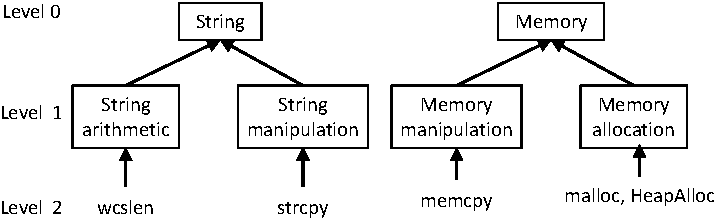
\includegraphics[height=3.5cm, width=8.5cm]{srj-figures/srj-abs-1.pdf} \vspace{-1mm}
\caption{System API abstraction levels}
\label{fig:abs} \vspace{-1mm}
\end{center}
\end{figure}

From Fig.~\ref{fig:abs}(a) and \ref{fig:abs}(b), it can be seen that based on the requirement of the analyst, there can be several ways to abstract a system API. That is, as shown in Fig.~\ref{fig:abs}(b), abstraction level 1 can be more expressive in providing more meaningful information about the API or it can be limited as in Fig.~\ref{fig:abs}(a). One of the key applications of abstraction level 0 is that it is mostly used in pre-filtering process, where if a signature involve string manipulation operation then it is wise to filter the target programs that involve in string manipulation. Similarly, abstraction level 1 is used to precisely match the signature with the target programs, where it can be used to specify additional constraints for the matching process. This is very useful for vulnerability signature matching, where for example, the analyst can remove functions, from the filtered target programs, that use secure system API (e.g., \texttt{strncpy}, \texttt{\_\_strncpy\_chk, $\ldots$}\footnote{With \texttt{FORTIFY\_SOURCE} compiler feature, whenever possible, \texttt{gcc} tries to uses buffer-length aware replacements for functions like \texttt{strcpy}, \texttt{memcpy}, \texttt{memset}, \texttt{gets}, $\ldots$, which are more secure.}), which are less likely to contain an exploitable vulnerability.

\subsubsection{Dependency Calculation} \label{subsubsec:dep_cal}
Algorithm \ref{algo:def-use} presents the steps involved in identifying the data dependence between assembly instructions. Here, we define several functions to accomplish our tasks. They are; (1) $\mathtt{getDef(i)}$ returns the variables defined in instruction $i$ (e.g., in `$\mathtt{mov\;eax,ebx}$', the register $\mathtt{eax}$ is defined), (2) $\mathtt{getUse(i)}$ returns the variables used in instruction $i$ (e.g., in the previous instruction, the register $\mathtt{ebx}$ is used), (3) $\mathtt{isPresent(g,G)}$ check whether the data-flow path $g$ is already present in $G$, where $G$ is a set of extracted data-flow paths, and (4) $\mathtt{getType(i)}$  returns the type of the instruction $i$. \note{At high-level, for each instruction present in the partial trace, we get the variables defined by that instruction and later, iterate through the rest of the instructions to check whether those defined variables are used elsewhere, if found, data dependency between those two instructions is established. Each iteration terminates either (1) reached end of partial trace, or (2) variable defined by instruction $i$ is redefined by another instruction $j$, where $location(i) < location(j)$. Finally, from each data-flow path in $G$, we check for the idioms that are extracted using Algorithm~\ref{algo:idiom-ext}}.

\begin{MyAlgo}[!ht]{-4.9cm} %increase or decrease margin, span across columns
 \DontPrintSemicolon
 \KwData{partial trace $\wp$}
 \KwResult{set of data-flow paths $G$}
% \SetKwFunction{algo}{ExtractTracelets}\SetKwFunction{proc}{Extract}
% \SetKwProg{myalg}{Algorithm}{}{}
% \myalg{\algo{$CFG$}}{
  $G \longleftarrow \emptyset$ \;%\tcp*{set of abstract semantic graphs}
 \ForEach{{\upshape instruction} i {\upshape in} $\wp$}{
  %\tcc{write the algo here}
  %$kT \longleftarrow kT \cup Extract(b, k)$\;
  $D_i \longleftarrow  \mathtt{getDef}(i)$\;
  $g \longleftarrow \emptyset$\;
  $j := i.\mathtt{Next}$\tcp*{$j$ is the next instruction after $i$ in $\wp$}
   \ForEach{{\upshape instruction} j {\upshape in} $\wp$}{
   $U_j \longleftarrow  \mathtt{getUse}(j)$\;
   $D_j \longleftarrow  \mathtt{getDef}(j)$\;
   \If{$U_j \in D_i $}{
	   	$g := g \cup {v_i \rightarrow v_j}$\;
   		 \If{$\mathtt{getType}(j) == \mathtt{DATA\_MOVEMENT}$}{
   			$D_i := D_i \cup D_j$\;
   		}
     }
      \If{$D_j \in D_i $}{
	   	$D_i := D_i \setminus D_j$\;
   		}
   		\If{$D_i ==  \emptyset $}{
   			%\If{$g$ {\upshape not in}  $G$}{
   			\If{$\mathtt{isPresent}(g,G) = 0$}{
   		 		$G := G \cup g$\;
   		 	}
	   	   $break$\;
   		}
   }
  }
  \Return ${G}$
  \\
 \caption{Data-flow analysis among instructions using def-use chain \note{seems there is a logic mistake, need to fix }}\label{algo:def-use}
\end{MyAlgo}



\subsubsection{Architecture and Platform Mapping} \label{subsubsec:archi_plat_dep}
It is observed that idiom extraction process is architecture and platform dependent task. That is, an idiom that is identical in-terms of high-level behaviour is implemented using completely different ISAs (Instruction Set Architectures)in different architectures, where each ISA has its own instruction set, register structure and addressing modes. For example, consider the following function prologues for ARM and x86 32bit architectures (We omitted the register normalization for the ease of understanding):

\begin{figure}[!th]
\scriptsize
  \begin{subfigure}[b]{0.5\linewidth}
   \centering
   % \includegraphics[width=0.75\linewidth]{srj-figures/srj-hierarchy-2.png}
    \raggedright{\textbf{\texttt{
    \\
    	mov ip, sp\\
    	stm sp!, {fp,ip,lr,pc}\\
    	sub fp, ip, Imm\\
    }}}
    \caption{\small{}}
   \label{fig:idiom2-ex-a}
    \vspace{1ex}
  \end{subfigure}%%
   \begin{subfigure}[b]{0.5\linewidth}
   \centering
   % \includegraphics[width=0.75\linewidth]{srj-figures/srj-hierarchy-2.png}
    \raggedright{\textbf{\texttt{
    \\
    	push ebp\\
    	mov ebp,esp\\
    	sub esp,Imm\\
    }}}
    \caption{\small{}}
   \label{fig:idiom2-ex-b}
    \vspace{1ex}
  \end{subfigure}%%
  \caption{Function prologue (i.e., stack frame set-up) for ARM and x86 32bit architectures.}
  \label{fig:idiom2-ex}
\end{figure}
From Fig.~\ref{fig:idiom2-ex-a} and \ref{fig:idiom2-ex-b}, it can be seen that ARM and x86 use completely different set of instruction sequence to set-up the stack frame in the function prologue. Further, to make things worst, even within the same architecture family the implementation conventions can drastically vary. For example, in x86-32 (IA-32), the function parameters are passed through the stack, however, in x86-64 (IA-64 or AMD64), the first several function parameters are passed using the registers and the rest are passed through the stack. Unfortunately, this discrepancy does not stops there. It gets even complicated across platforms, where for the same architecture different platforms have different ABIs (Application Binary Interface). For example, for non-float/double parameter passing, in x86-64, Microsoft ABI uses the registers \texttt{rcx}, \texttt{rdx}, \texttt{r8} and \texttt{r9}, whereas, system V ABI (the ABI Linux uses) uses the registers \texttt{rdi}, \texttt{rsi}, \texttt{rdx}, \texttt{rcx}, \texttt{r8} and \texttt{r9}.

\begin{table*}[!th]
	\begin{center}
  \begin{tabular}{|c|c|c|c|}
  \hline
  \rule[-1ex]{0pt}{2.5ex} \textbf{Idiom Type} & \textbf{Actual Implementation} & \textbf{Idiom} & \textbf{High-level meaning} \\
  \hline
  \rule[-1ex]{0pt}{2.5ex} \textbf{Semantic idiom} & ? & ? & ? \\
  \hline
  \rule[-1ex]{0pt}{2.5ex} \textbf{Structural idiom} & {push ebp;	mov ebp,esp; 	sub esp,0x32;} & {push ebp;	mov ebp,esp; 	sub esp,0x32;} & Stack frame set-up in function prologue \\
  \hline
  \rule[-1ex]{0pt}{2.5ex} \textbf{Compiler idiom} & ? & ? & ? \\
  \hline
  \end{tabular}
   \vspace{2ex}
  \caption{Non-exhaustive list of extracted idioms. their actual implementation and the high-level meanings. \note{give 3 examples for each idiom type}}\label{tab:idiom_list}
  \end{center}
\end{table*}

Hence, in \tool, we work with high-level behaviour of idioms which are unified across different platforms and architectures. It is important to note that the function normalization process presented in Section~\ref{subsubsec:func_norm} is x86 architecture specific, however, similar approach is adapted, with some modifications,to normalize ARM instructions. For example, ARM has different addressing modes compare to x86 and it needs to be properly handled normalization process. Table \ref{tab:idiom_list}, presents a non-exhaustive list of idioms extracted and their high-level meaning (or behaviour) for each idiom type.
